\subsection{Formula1 Live}
%link all'articolo:
% http://www.f1world.it/formula-1-live/

Verrà analizzata la pagina relativa alle informazioni sui tempi delle sessioni
di una gara di Formula1.

\begin{figure}[H] % 'h' not 'H'
  \centering
  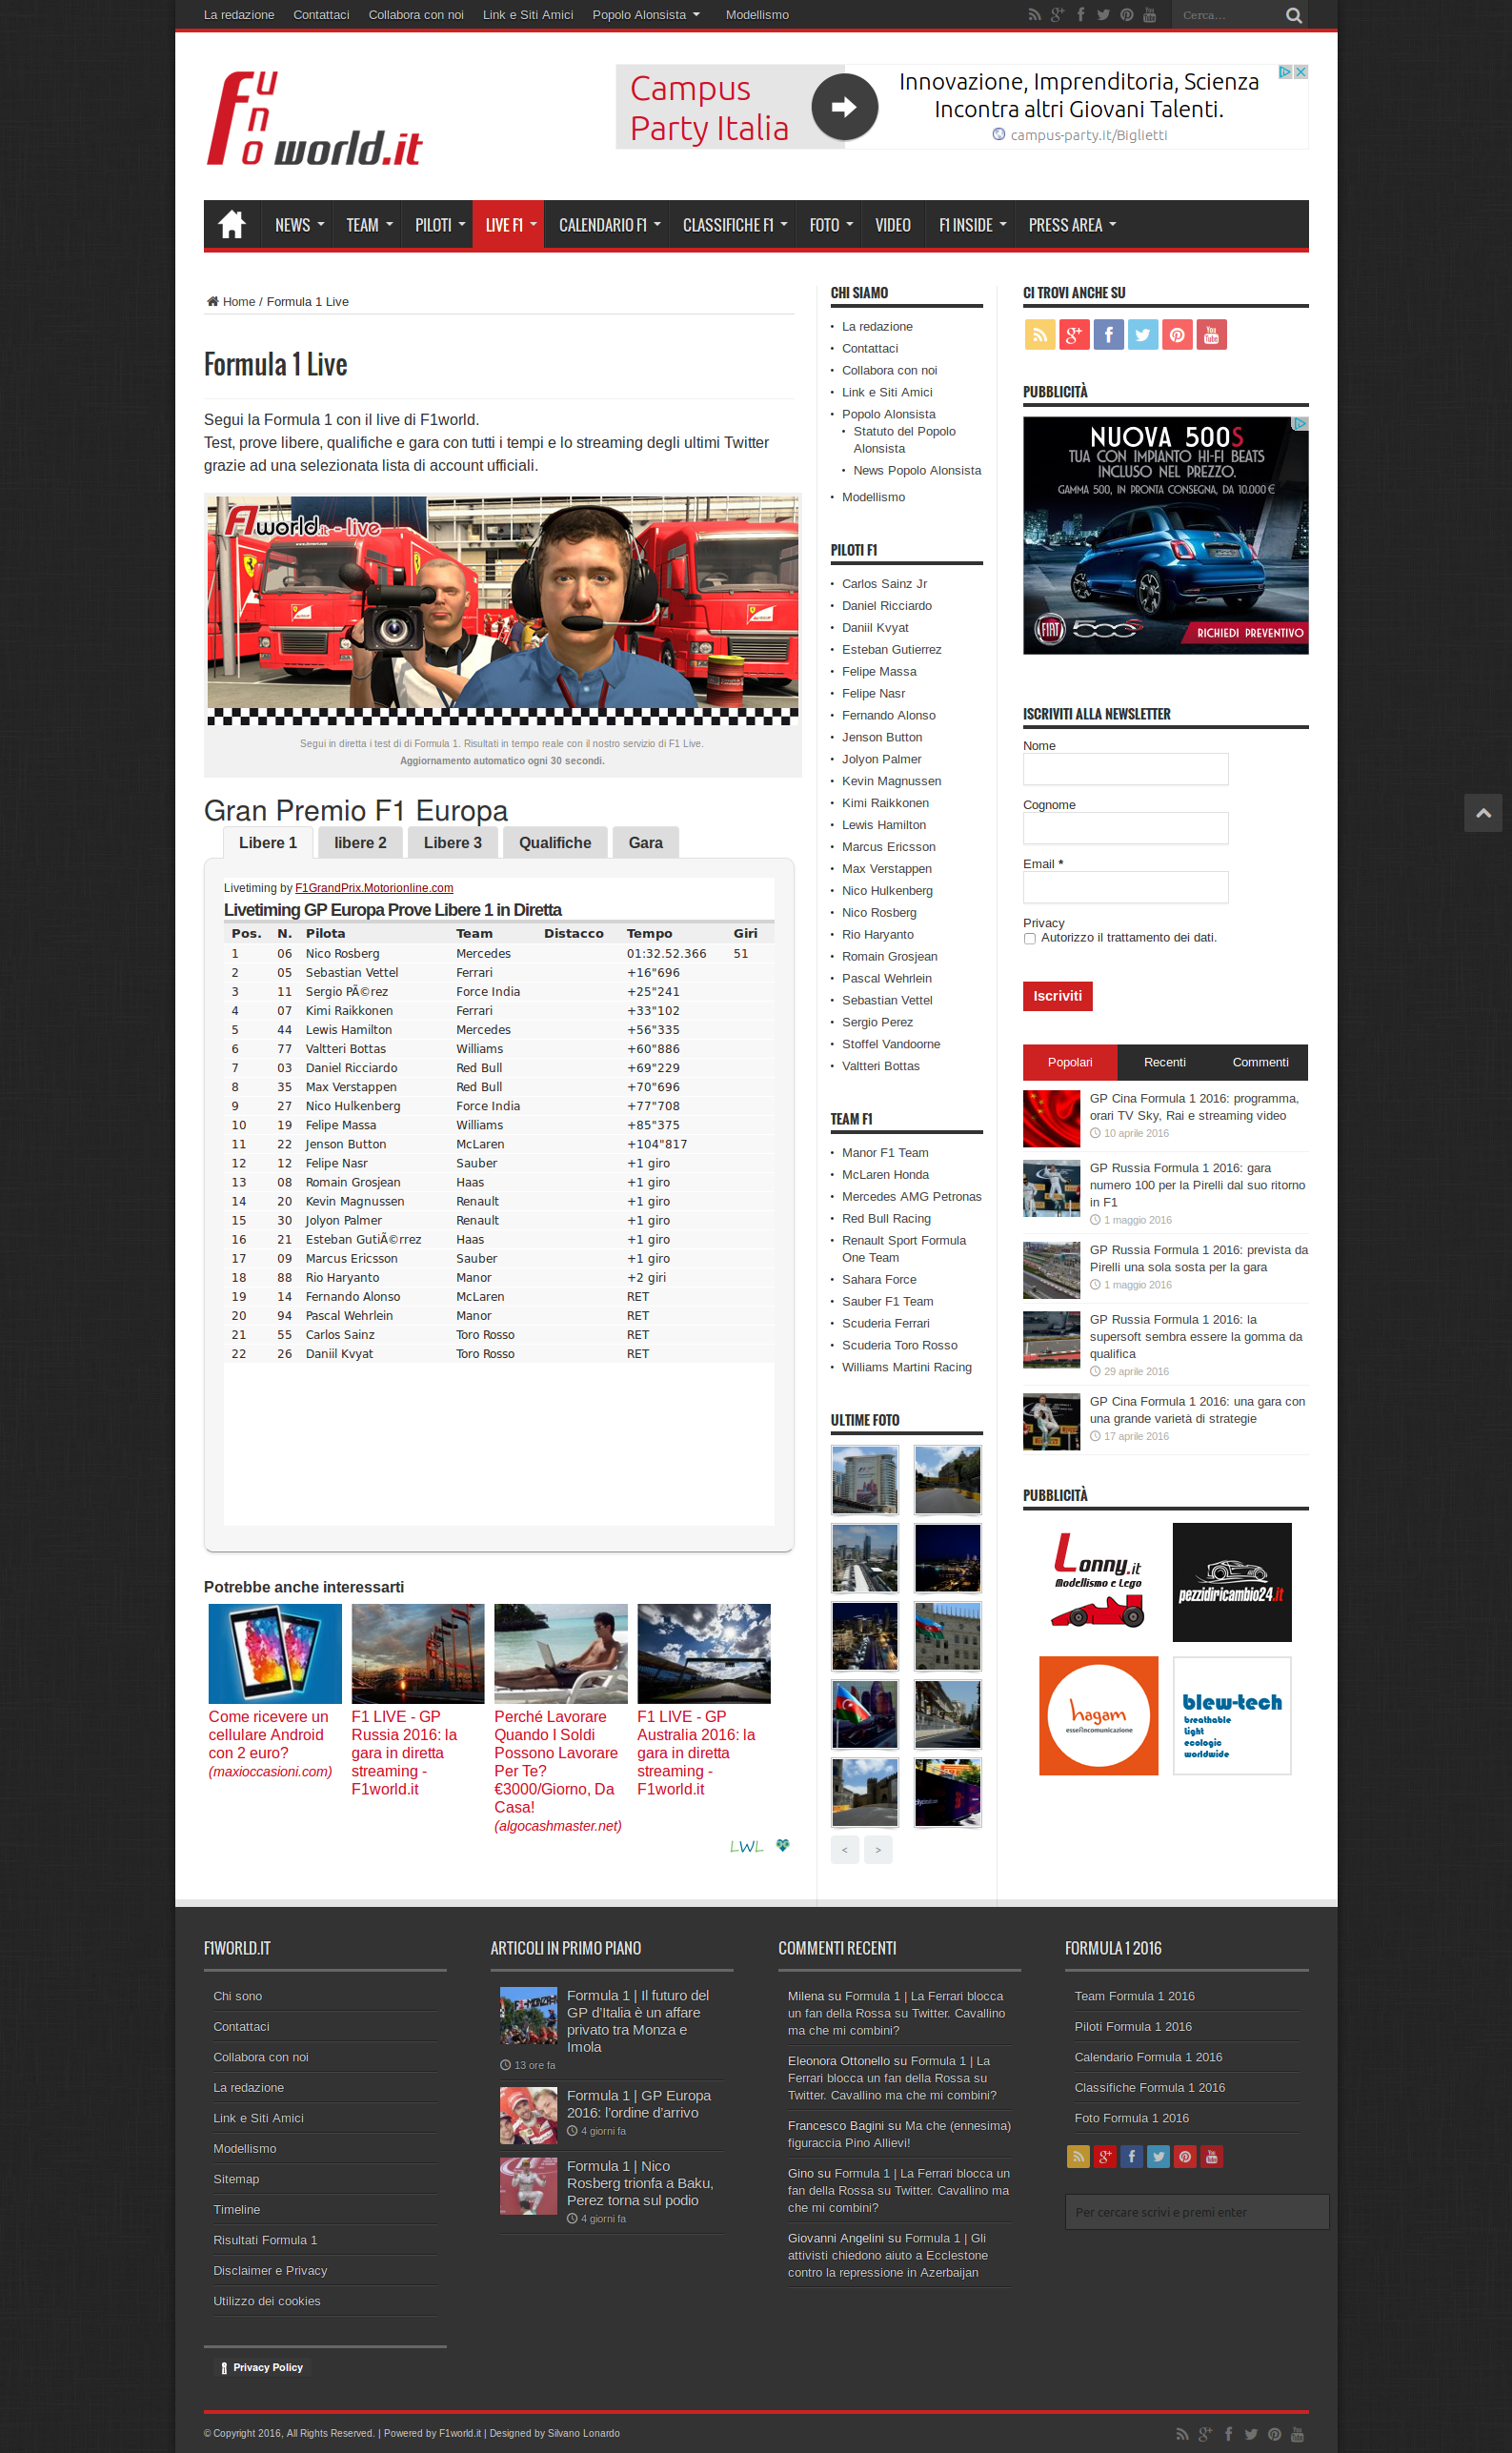
\includegraphics[height=18cm, width=10cm]{res/img/Formula1Live_Full}
  \caption{\textit{Screenshot} della sezione ``Formula1 Live''}
\end{figure}

Questa pagina presenta diversi difetti a livello di usabilità.
Innazitutto è presente un'immagine (che potrebbe essere a mio avviso
migliorabile) all'inizio del contenuto, che aumenta il numero di scroll. Inoltre
questa pagina non risulta utile ai fini del contenuto stesso, occupando solo
spazio.

Scendendo nella pagina possiamo trovare il contenuto: una tabella suddivisa per
schede. Per ogni scheda è presente la classifica della sessione, che si aggiorna
in tempo reale. Questa tabella presenta problemi relativi ai caratteri
accentati, che non vengono visualizzati correttamente.

Riguardo al contenuto, è possibile vedere come la scheda ``Prove libere''
sia uguale alle informazioni presenti nella scheda ``Gara''. Questo problema
causa all'utente disorientamento, in quanto dovrebbe aspettarsi di vedere
informazioni diverse sui tempi in base alla sessione selezionata.

\begin{figure}[H]

  \centering
  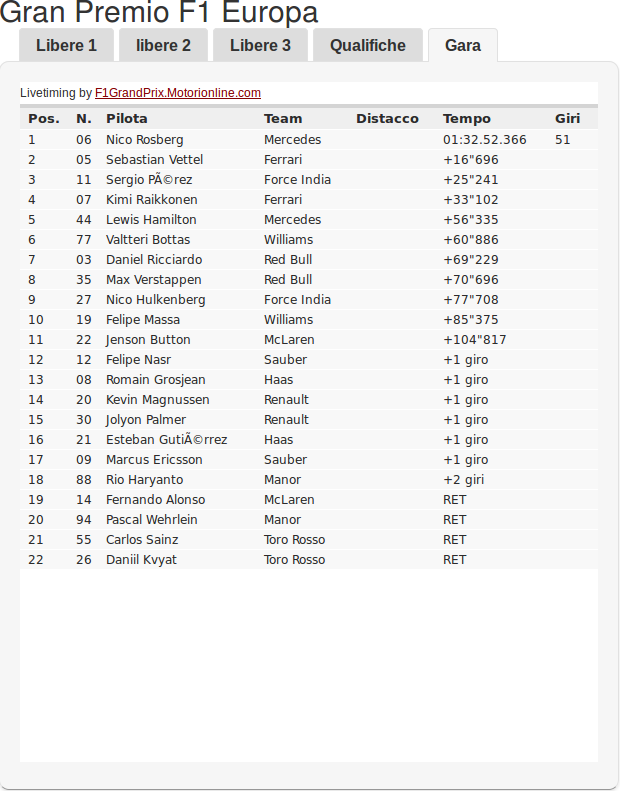
\includegraphics[scale=0.5]{res/img/dettagli/tableScore}
  \caption{Scheda ``Gara'', che risulta essere uguale a ``Prove libere''
    presenti nello \textit{screenshot} di tutta la pagina} 
\end{figure}

La pagina presenta un altro difetto globale: ogni 30 secondi viene eseguito un
\textit{refresh} automatico, senza possibilità di annullarlo. Questo genera
molta frustazione all'utente, che si vede ogni 30 secondi ricaricarsi la pagina.

Finito il contenuto è presente una sezione di articoli a riguardo, in cui sono
presenti annunci pubblicitari.
